\documentclass[10pt,compress]{beamer}
\usepackage{amsmath}
\usepackage{url}
\usepackage{ucs}
\usepackage[utf8x]{inputenc}
\usepackage[ngerman]{babel}
\usepackage{ulem}  % sout
\usepackage{multicol}
\usepackage{setspace}
\usepackage{bookman}

\title{Embedded Linux am Beispiel des Gnublin-Boards}
\date{7. November 2012}

\usetheme{Warsaw}  %Warsaw, Berkeley?
\usecolortheme{seahorse}
\usefonttheme{serif}
\useinnertheme{rectangles}
\setbeamercovered{transparent}

\begin{document}

\frame{
  \begin{center}
    \huge Embedded Linux am Beispiel des Gnublin-Boards

    \vfill

    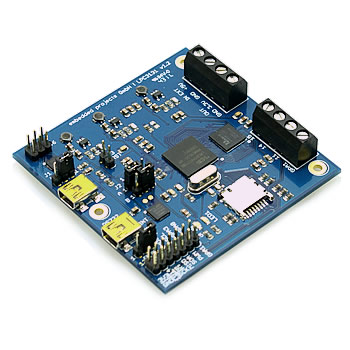
\includegraphics[scale=0.4]{gnublin.jpg}
  \end{center}
}

\section{Embedded Linux}
\frame {
  \frametitle{Was ist Embedded Linux?}

  \begin{block}{Wikipedia}
    Als Embedded Linux bezeichnet man ein eingebettetes System mit einem auf dem Linux-Kernel basierenden Betriebssystem.
  \end{block}

% \pause

  In der Praxis:
  \begin{itemize}
    \item Board mit Prozessor (z.B. ARM, MIPS), RAM und externen Schnittstellen
    \item oftmals Graphik-Prozessor und Display integriert
    \item Sensoren, Akku als Spannungsversorgung
    \item stromsparend, klein, leise, günstig
    \vfill
% \pause
    \item Einsatzgebiete:
    \begin{itemize}
     \item kleiner Server (Router)
     \item für Steuer- und Regelaufgaben (Drohnen, Segways)
     \item Automatisierung (Rolladen, Beleuchtung, Kaffeemaschine)
     \item Unterhaltungselektronik (Media-Player)
     \item Handys (Android)
     \end{itemize}
  \end{itemize}
}

\frame {
  \frametitle{Embedded Linux}

  Was braucht man für die Hardware?
  \begin{itemize}
    \item Prozessor auf dem Linux läuft
    \item RAM
    \item Speicherplatz (z.B. NAND, SD-Karte)
    \item Schnittstellen / IO-Ports / Display $\dots$
  \end{itemize}

  \vfill
% \pause

  Was braucht man an Software?
  \begin{itemize}
    \item auf dem PC: 
    \begin{itemize}
      \item Cross-Compiler (gcc)
      \item Tool zum Übertragen der Software / Firmware
    \end{itemize}
    \item auf dem Embedded Linux System:
    \begin{itemize}
      \item Bootloader
      \item Linux-Kernel
      \item Linux-System (initramfs, root-Dateisystem)
    \end{itemize}
  \end{itemize}
}

\section{gnublin Board}

\frame {
  \frametitle{Motivation}

  \begin{itemize}
    \item entwickelt von \href{http://www.embedded-projects.net}{Embedded Projects GmbH} in Zusammenarbeit mit der Hochschule Augsburg
    \item Board mit zwei Lagen
  \end{itemize}

  Ziele
  \begin{itemize}
    \item günstiges Embedded Linux Board für Ausbildung
    \item einfacher Einstieg ohne große Vorkenntnisse
    \item ein einfaches USB Kabel soll ausreichen
    \item freie Lizenz für Hard- und Software
    \item Preis nicht höher als 50 Euro
    \item Unterstützung vieler Programmiersprachen
    \item Einfaches soll einfach, komplexe Aufgaben möglich sein
    \item gute Dokumentation
  \end{itemize}
}

\frame {
  \frametitle{Hardware}

  \begin{itemize}
  \item 180 MHz ARM9 / 32 MB RAM
  \item USB serielle Konsole On-Board (CP2102)
  \item Stromversorgung per USB oder Netzteil 7-12V
  \item microSD Karte
  \item 3x IO, 3x AD extern an Anschlussklemme
  \item I2C, SPI und UART
  \item USB Device oder Host (OTG)
  \item drei Versionen: Standard, Extended, DIP
  \end{itemize}

  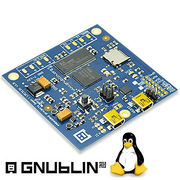
\includegraphics[scale=0.35]{standard.jpeg}
  \hfill
  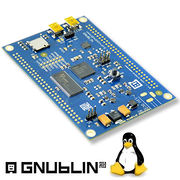
\includegraphics[scale=0.35]{extended.jpeg}
  \hfill
  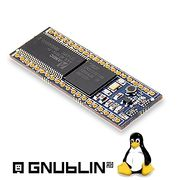
\includegraphics[scale=0.35]{dip.jpeg}
}

\frame {
  \frametitle{Hardware -- Komponenten}

  \begin{center}
  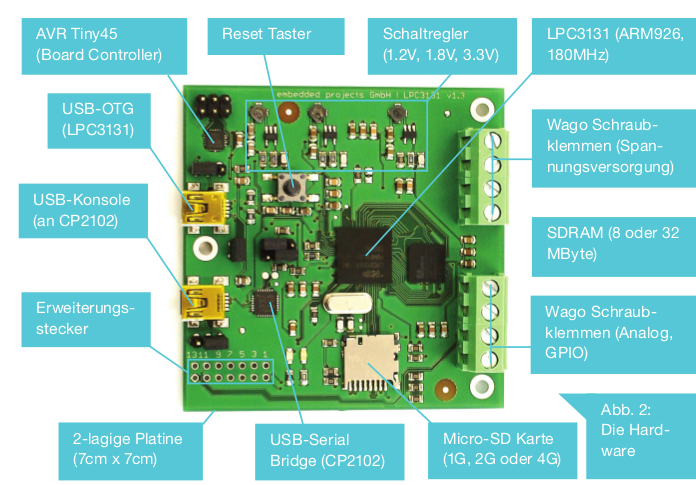
\includegraphics[scale=0.35]{komponenten.png}
  \end{center}
}

\frame {
  \frametitle{Schnellstart}

  \begin{enumerate}
    \item SD-Karte mit root-Dateisystem und Kernel in den Halter stecken
    \item Gnublin über USB-Kabel mit Strom versorgen (RS232 Buchse)
    \item Terminalemulator starten (z.B. picocom)
    \item Linux-System benutzen
  \end{enumerate}

  \begin{center}
  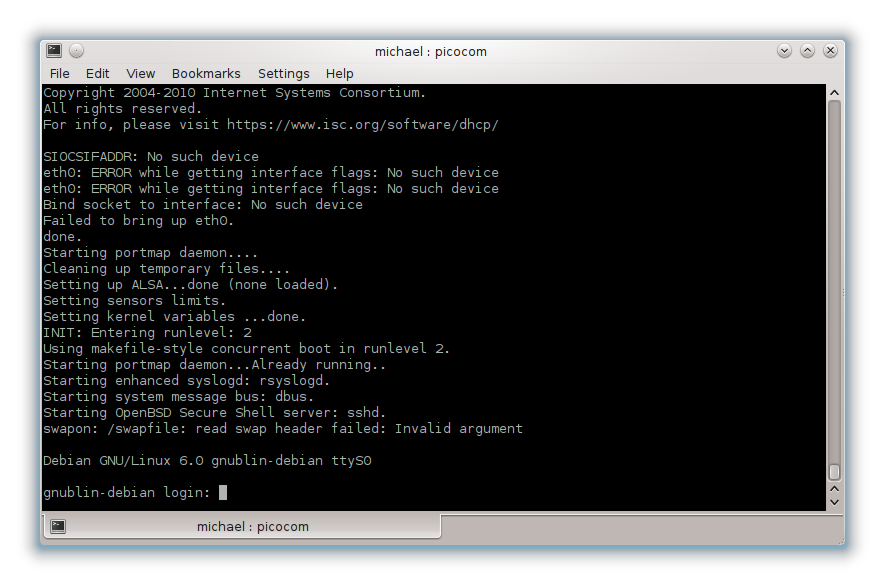
\includegraphics[scale=0.3]{bootup.png}
  \end{center}
}

\frame {
  \frametitle{Software-Komponenten}

  \begin{itemize}
    \item Bootloader: apex
    \begin{itemize}
      \item viele integrierte Kommandos
      \item Erweiterung über neue Kommandos einfach möglich
    \end{itemize}

    \vfill

    \item Kernel: Linux 2.6.33
    \begin{itemize}
      \item neuere Kernel sollten ohne große Anpassungen nutzbar sein
      \item Kernel mit Real Time Patches verfügbar
      \item Kernel durch eigene Kernel Module erweiterbar
      \item initramfs kann ebenfalls benutzt werden
    \end{itemize}
    
    \vfill

    \item root-Dateisystem
    \begin{itemize}
      \item Debian mit vielen Paketen
      \item Pakete nachinstallierbar
    \end{itemize}
  \end{itemize}
}

\frame {
  \frametitle{USB}

  gnublin als USB-Device
  \begin{itemize}
    \item gnublin kann als USB-Device verwendet werden
    \item viele USB-Gadgets verfügbar unter Linux:
    \begin{itemize}
      \item g\_ether:         Ethernet emulation on USB
      \item g\_file\_storage: Mass storage
      \item g\_serial:        Serial emulation on USB
    \end{itemize}
  \end{itemize}

  \vfill

  gnublin als USB-Host:
  \begin{itemize}
    \item an gnublin können beliebige USB-Geräte angeschlossen werden
    \item allerdings USB-Host Adapter notwendig (ca. 2 Euro)
    \item z.B.: Webcam, WLAN, LAN, Massenspeicher, Audio
  \end{itemize}
  \hfill 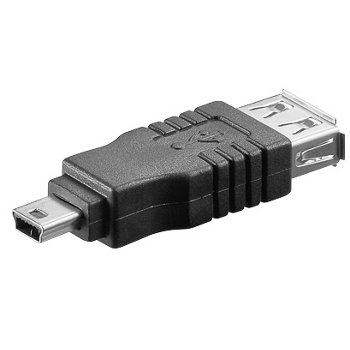
\includegraphics[scale=0.15]{adapter.jpeg}
}

\section{Programmieren}
\frame {
  \frametitle{Programmiersprachen}

  Alle unter Linux verfügbaren Programmiersprachen:

  \begin{itemize}
    \item C, C++
    \begin{itemize}
      \item Crosskompilierung auf dem PC (arm-linux-gnueabi-gcc)
      \item Cross-Compiler kann durch einfaches Entpacken installiert werden
      \item natives Kompilieren direkt auf dem Board (langsam, bei kleinen Programmen aber ohne Probleme möglich)
    \end{itemize}
    \item Skriptsprachen
    \begin{itemize}
      \item Python
      \item Perl
      \item Lua (spartanisch und sehr schnell)
      \item PHP
      \item Ruby
      \item Bash, Shell
    \end{itemize}
    \item Go
    \item theoretisch auch Java
  \end{itemize}
}

\frame {
  \frametitle{Zugriff auf Hardware}

  \begin{itemize}
    \item Alles ist eine Datei!
    \item z.B.: Ansteuern der GPIOs über sysfs:
    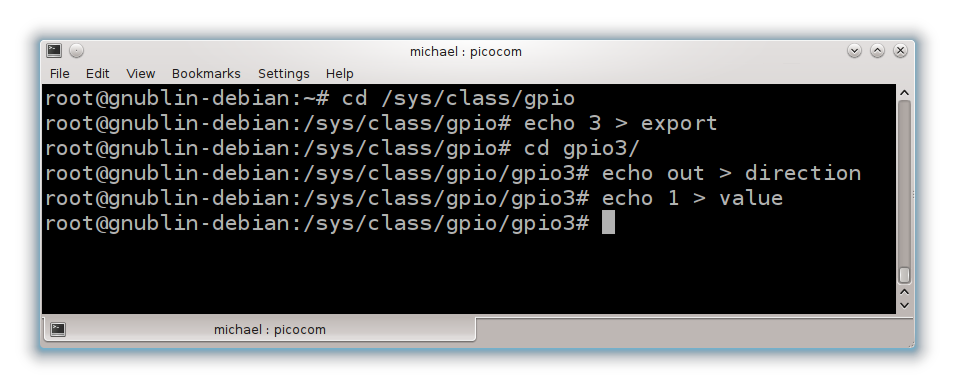
\includegraphics[scale=0.41]{gpio.png}
    \item I2C, SPI, ADC, UART ähnlich
    \item Zugriff von allen Programmiersprachen aus möglich
  \end{itemize}
}

\frame {
  \frametitle{Anwendungen}

  Was kann man jetzt damit machen?
  \begin{itemize}
    \item gnublin über WLAN-Stick mit dem eigenen Netzwerk verbinden
    \item Steuerung von Rolläden, Beleuchtung, Kaffeemaschine über Relais zu bestimmten Zeiten bzw. über Webinterface
    \vfill
    \item auch denkbar als Steuerung für Roboter oder Drohne
    \item gnublin steuert Motoren, überwacht Sensoren
    \item Webcam zeigt Bilder, GPS liefert aktuelle Position
    \item Roboter/Drohne lässt sich über WLAN steuern
  \end{itemize}

  \hfill 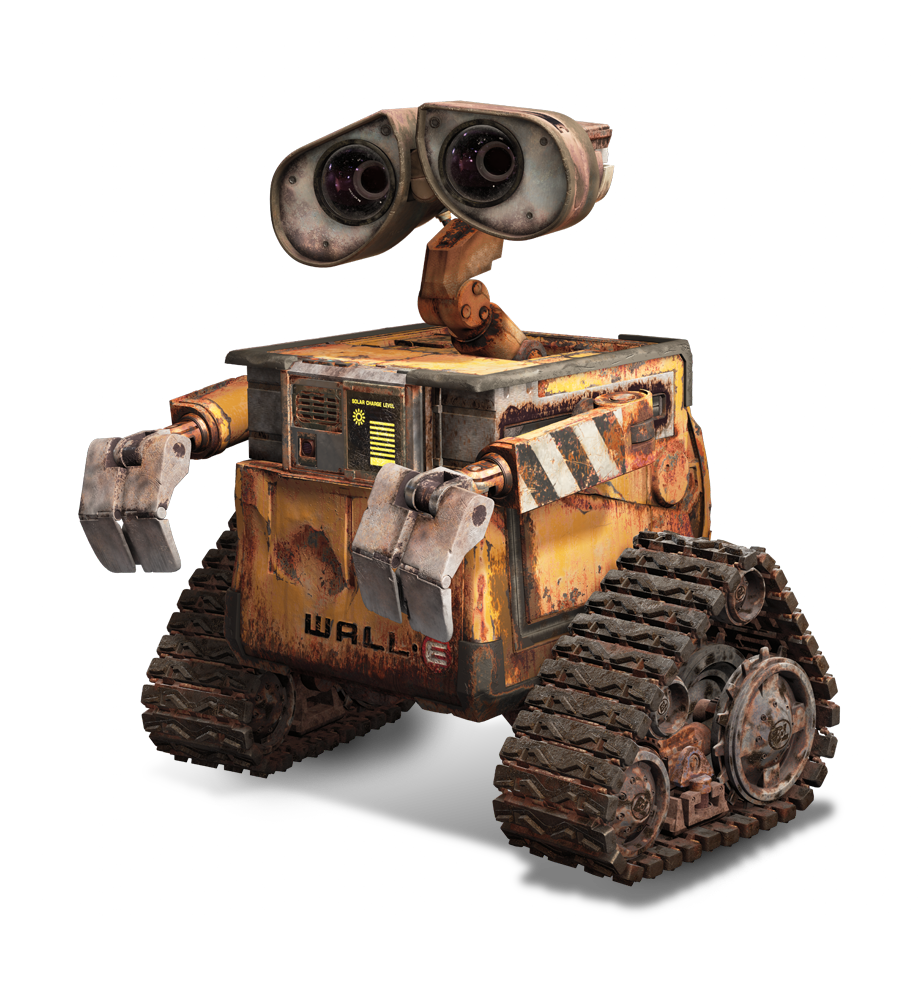
\includegraphics[scale=0.065]{walle.png}
}

\section{Sonstiges}
\frame {
  \frametitle{Vielen Dank!}

  \begin{center}
  { \huge Vielen Dank für Eure\\\  \\Aufmerksamkeit! }
  \end{center}

  \vfill
  
  Weitere Informationen finden sich unter \href{http://wiki.gnublin.org}{wiki.gnublin.org}.
}

\end{document}
